%% This is file `elsarticle-template-1-num.tex',
%%
%% Copyright 2009 Elsevier Ltd
%%
%% This file is part of the 'Elsarticle Bundle'.
%% ---------------------------------------------
%%
%% It may be distributed under the conditions of the LaTeX Project Public
%% License, either version 1.2 of this license or (at your option) any
%% later version.  The latest version of this license is in
%%    http://www.latex-project.org/lppl.txt
%% and version 1.2 or later is part of all distributions of LaTeX
%% version 1999/12/01 or later.
%%
%% The list of all files belonging to the 'Elsarticle Bundle' is
%% given in the file `manifest.txt'.
%%
%% Template article for Elsevier's document class `elsarticle'
%% with numbered style bibliographic references
%%
%% $Id: elsarticle-template-1-num.tex 149 2009-10-08 05:01:15Z rishi $
%% $URL: http://lenova.river-valley.com/svn/elsbst/trunk/elsarticle-template-1-num.tex $
%%
%%\documentclass[preprint,12pt]{elsarticle}

%% Use the option review to obtain double line spacing
%% \documentclass[preprint,review,12pt]{elsarticle}

%% Use the options 1p,twocolumn; 3p; 3p,twocolumn; 5p; or 5p,twocolumn
%% for a journal layout:
%% \documentclass[final,1p,times]{elsarticle}
%% \documentclass[final,1p,times,twocolumn]{elsarticle}
%% \documentclass[final,3p,times]{elsarticle}
 \documentclass[final,3p,times,twocolumn]{elsarticle}
%% \documentclass[final,5p,times]{elsarticle}
%% \documentclass[final,5p,times,twocolumn]{elsarticle}

%% if you use PostScript figures in your article
%% use the graphics package for simple commands
%% \usepackage{graphics}
%% or use the graphicx package for more complicated commands
%% \usepackage{graphicx}
%% or use the epsfig package if you prefer to use the old commands
%% \usepackage{epsfig}

%% The amssymb package provides various useful mathematical symbols
\usepackage{amssymb}
%% The amsthm package provides extended theorem environments
%% \usepackage{amsthm}

%% The lineno packages adds line numbers. Start line numbering with
%% \begin{linenumbers}, end it with \end{linenumbers}. Or switch it on
%% for the whole article with \linenumbers after \end{frontmatter}.
%% \usepackage{lineno}

%% natbib.sty is loaded by default. However, natbib options can be
%% provided with \biboptions{...} command. Following options are
%% valid:

%%   round  -  round parentheses are used (default)
%%   square -  square brackets are used   [option]
%%   curly  -  curly braces are used      {option}
%%   angle  -  angle brackets are used    <option>
%%   semicolon  -  multiple citations separated by semi-colon
%%   colon  - same as semicolon, an earlier confusion
%%   comma  -  separated by comma
%%   numbers-  selects numerical citations
%%   super  -  numerical citations as superscripts
%%   sort   -  sorts multiple citations according to order in ref. list
%%   sort&compress   -  like sort, but also compresses numerical citations
%%   compress - compresses without sorting
%%
%% \biboptions{comma,round}

% \biboptions{}

% HPS stuff
\usepackage{color}
%\usepackage{multicol}
\newcommand{\Aprime}{A\ensuremath{^\prime}}
\newcommand{\ee}{e$^+$e$^-$}
\newcommand{\fluenceunit}{1~MeV~neutron~equivalent/cm\ensuremath{^2}}
\newcommand{\geant}{{\sc Geant4}}
\newcommand{\egs}{{\sc EGS5}}
\newcommand{\moliere}{Moli\`{e}re}


\journal{Nuclear Physics B}

\begin{document}

\begin{frontmatter}

%% Title, authors and addresses

%% use the tnoteref command within \title for footnotes;
%% use the tnotetext command for the associated footnote;
%% use the fnref command within \author or \address for footnotes;
%% use the fntext command for the associated footnote;
%% use the corref command within \author for corresponding author footnotes;
%% use the cortext command for the associated footnote;
%% use the ead command for the email address,
%% and the form \ead[url] for the home page:
%%
%% \title{Title\tnoteref{label1}}
%% \tnotetext[label1]{}
%% \author{Name\corref{cor1}\fnref{label2}}
%% \ead{email address}
%% \ead[url]{home page}
%% \fntext[label2]{}
%% \cortext[cor1]{}
%% \address{Address\fnref{label3}}
%% \fntext[label3]{}

\title{The Heavy Photon Search Test Detector}

%% use optional labels to link authors explicitly to addresses:
%% \author[label1,label2]{<author name>}
%% \address[label1]{<address>}
%% \address[label2]{<address>}

\author[label1]{Per Ledin}
\ead{contact@hps.discovery.com}
%\author[slac]{Per Hansson Adrian\corref{cor1}}
%\ead{phansson@slac.stanford.edu}
%\author[slac]{Timothy K. Nelson}
%\address[slac]{SLAC National Accelerator Laboratory, 94025, Menlo Park, CA, USA}
\address[label1]{Lule\aa~Hockey}

\begin{abstract}
Heavy photons, aka "hidden sector" or "dark" photons, are massive cousins to the SM photon, 
which couple to an analogue of electric charge. They arise naturally in theories with additional
U(1) gauge groups, and have been proposed as a possible explanation for the muon g-2 anomaly,
astrophysical puzzles, and possible sightings of light dark matter in direct detection experiments.
Masses in the range 10 to 1000 MeV are suggested. Heavy photons couple weakly to electric charge, 
so can be produced via electroproduction and can decay into elecron-positron pairs, albeit at rates 
strongly suppressed compared to standard QED trident processes. Consequently, heavy photons must be identified
above copious backgrounds, requiring high luminosity/high rate experiments, good mass resolution
(to identify invariant mass bumps), and good vertexing (to see the long lifetimes implied by
weak couplings). The Heavy Photon Search (HPS) will use  a silicon microstrip vertex tracker
triggered by a high speed PbWO4 electromagnetic calorimeter to search 
for these states in a fixed target experiment at Thomas Jefferson National Accelerator Facility (JLab). 
The first stage of HPS was the HPS Test Run experiment, designed to demonstrate the technical feasibility of the detector and data
acquisition systems and to confirm that critical backgrounds were correctly modeled.
This paper describes the HPS Test Run detector, reviews its performance, and presents results of
the normalized trigger rate measurements that confirm the accuracy of the background simulation.
\end{abstract}

\begin{keyword}
%% keywords here, in the form: keyword \sep keyword
silicon microstrips \sep tracking  \sep vertexing \sep heavy photon \sep electromagnetic calorimeter
%% MSC codes here, in the form: \MSC code \sep code
%% or \MSC[2008] code \sep code (2000 is the default)

\end{keyword}

\end{frontmatter}

\tableofcontents
\clearpage
\newpage
\newpage

%%
%% Start line numbering here if you want
%%
% \linenumbers

%% main text
\section{Introduction}
\label{introduction}
One of the more striking anomalies in recent astrophysical observations is an excess of high energy electrons and positrons consistent with a large, unknown source of pair production~\cite{Adriani:2008zr}\cite{FermiLAT:2011ab}. The existence of a massive, hidden sector vector boson; a ``dark photon;" that mixes kinetically with the Standard Model photon and mediates annihilation or decay of dark matter particles is a theoretically attractive explanation of this cosmic-ray excess~\cite{Holdom:1985ag}\cite{ArkaniHamed:2008qn}.
\begin{center}
{\small
\begin{figure*}[ht]
    \includegraphics[width=0.8\textwidth]{figures/hps_testrun_rendering}
\caption{Rendering of the HPS Test apparatus installed on the beam line.}
\label{fig:testrundetector}
\end{figure*}
}
\end{center}

Heavy photons, aka known as "hidden sector" or "dark" photons, are particles with mass 10-1000 MeV which 
couple
weakly to the SM photon, so can be radiated by electrons, and can decay into e+e- pairs, albeit at rates far
below those of QED trident processes. They have been suggested by numerous Beyond Standard Model 
theories and
as an explanation of the current muonic g-2 anomaly, and may couple directly
to hidden sector particles that may constitute all or some of the dark matter. Current phenomenology highlights 
the 
20-1000 MeV mass range, and suggests that heavy photons couple to electric charge with strength 
$\epsilon$e, where 
$\epsilon$ is in the range of $10^{-3} -10^{-5}$. This range of parameters makes heavy photon searches viable 
at electron-positron colliders and in moderate energy fixed target electroproduction, and results from both
approaches have already been reported. Fixed target experiments offer the highest sensitivity 
for heavy photons with mass $<1000$~MeV~\cite{Bjorken:2009mm}, but require large data sets and good 
mass resolution to identify a small mass peak above the copious QED background. At small couplings, heavy 
photons become long-lived, so detection of a secondary decay vertex can reject the prompt QED background 
and boost experimental sensitivity.
The HPS experiment uses both invariant mass and vertex signatures by placing a compact silicon tracking and 
vertexing detector ($\approx 1$~m long) immediately downstream ($\approx 10$~cm) of a thin target 
($\approx0.25~X_0$ tungsten) and inside of a dipole magnet ($\approx 1$~T)~\cite{HPS_proposal_2010}. 
The experiment runs at high rates, exploiting the 100\% duty cycle of the 
CEBAF accelerator to accumulate the need statistics. The trigger is provided by a fast electromagnetic 
calorimeter just downstream of the magnet.


The HPS Test run, a simplified version of the full HPS experiment, was proposed and approved at JLab 
as the first stage of the HPS experiment.  Its purposes included demonstrating that the apparatus and data 
acquisition systems are technically feasible and
that the trigger rates and occupancies encountered in electron-beam running are as simulated. Additionally,
given dedicated running time with electron beams, the HPS Test Run could provide new sensitivity to heavy 
photons. The HPS Test apparatus was installed on April 19, 2012, and 
ran parasitically with the HDice experiment, using its photon beam, until May 18. The JLab run schedule 
precluded any dedicated electron beam running, but the HPS Test Run was allowed a short and valuable
dedicated run with the photon beam.

This paper reviews the HPS Test Run apparatus. It documents the successful performance of the trigger, data 
acquisition, silicon tracker, and ECal and
shows that the performance assumed in calculating the physics reach of the experiment is realistic.
Of particular importance, data from the dedicated photon beam running has been used to compare
the measured trigger rates with those expected in simulation. The Test Run trigger rate is almost entirely due to
photons which have converted to \ee{} pairs in a thin target upstream of HPS and it is sensitive to the particulars 
of their multiple Coulomb scattering in the conversion target.  Since, during electron beam running, the tails of 
the multiply Coulomb scattered primary beam are the dominant source of occupancy in the tracker and the 
trigger rate in the Ecal, they must be understood quantitatively. The trigger rates in the Test Run are also 
sensitive to the tails of the multiple Coulomb scattering distribution. Good agreement between the measured 
and simulated rates confirms our understanding of multiple Coulomb scattering and 
the reliability of the background simulation used to benchmark the physics reach of the HPS experiment. 

The very small signal rate compared to the large background and the need to reconstruct the final states of 
the electron and positron in a dense radiation environment millimeters from a high-current beam 
place stringent requirements on the detector, which should have,
\begin{itemize}
\item large and uniform acceptance in the forward region to catch boosted decay products,
\item a flexible, redundant and efficient trigger selecting electron and positron pairs at rates up to 50kHz,
\item excellent track reconstruction efficiency for electrons and positrons,
\item good angular and momentum resolution to reconstruct invariant mass precisely,
\item excellent vertex resolution to search for displaced heavy photon decays,
\item high rate electronics with event timing resolution down to 2~ns,
\item data acquisition system capable of handling data rates of 100~MB/s to permanent storage,
\item detector components that can survive and efficiently operate in a high radiation environment with 
local doses exceeding $100$~Mrad
\end{itemize}












\section{Detector Overview}
\label{detector}
The HPS experiment is proposed to run in Hall B using electron beams of Continuos Electron Beam 
Accelerator Facility (CEBAF) at JLab. CEBAF can simultaneously deliver  electron 
beams to multiple experimental hall at 499 MHz frequency with beam currents of up to 150 $\mu$A (Hall-B 
is limited to $<1 ~\mu$A).  Currently CEBAF facilities are undergoing energy an upgrade that is expected to be 
completed in end of 2014. The upgraded CEBAF machine will double its maximum energy from $6$~GeV 
during the HPS test run to $12$~GeV. 


The HPS Test apparatus was designed as a 
first step of a multi-stage approach 
to the HPS experiment. The primary goal was to demonstrate that the technology and design approach 
chosen are sound for running in such a challenging environment. Nevertheless, a secondary but 
important aspect was that, after proving the technical concepts,  the apparatus would have the 
capability to discover \Aprime{} events. The implication was that the design of the HPS Test apparatus 
would be subject to almost the same constraints and requirements as the full experiment.
The kinematics of \Aprime{} production typically results in final state particles within a few degrees of the incoming beam, especially at low 
$m_{\Aprime{}}$.  
%Step
This implies that the apparatus for an \Aprime{} search in electron interactions with fix targets must operate in 
close proximity to an intense electron beam that passes through a high-Z target. 
Hence it should cope with high backgrounds and tolerate the high radiation environment. 
To meet this challenge, HPS will deploy high rate and radiation hard detector composed of 
a silicon vertex tracker with 40~MHz readout and a PbWO$_4$ crystal calorimeter with 250~MHz 
readout, capable of triggering multi-prong events at top to 50~kHz rate.


%\subsection{HPS Test setup}

The HPS Test apparatus, a simplified version of that 
planned for the full HPS experiment, demonstrates the feasibility of the detector
technologies proposed for the silicon tracker, electromagnetic calorimeter, and data acquisition system. 
A rendering of the HPS Test setup is shown in Fig.~\ref{fig:testrundetector}. The setup is based on the Hall-B 
pair spectrometer (PS) magnet, 18D36 dipole. The silicon vertex tracker (SVT) was installed inside the vacuum 
chamber of PS and the electromagnetic calorimeter (ECal) was mounted behind the vacuum flange. 
A new vacuum box 
attached to the upstream end of the pair spectrometer vacuum chamber provided necessary services to 
the SVT (cooling, power and signal readout). 
Most technologies used in the HPS Test apparatus as well as the magnet and the vacuum chamber will be 
used in the HPS detector with some 
improvements to each of the systems; both from lessons learned during running of the HPS Test but 
also from planned upgrades for longer and more effective running. 

%\begin{multicols}{2}
\begin{center}
\begin{table*}[t]
{\small
\caption{Overview of the coverage, segmentation and performance of the HPS Test detector. }
\begin{tabular}{lccccccc}
\hline 
System & Coverage & \# channels & ADC & Time resolution & \# layers & Segmentation & Performance \\
 & (mrad) &  & (bit) & (ns) &  &  &  \\
\hline
SVT & $15<\theta_{y} < XXXX$ & 12800 & 14 & $\approx 2$~ns & 5  & $\approx 120~\mu$m $r-\phi$ & $\sigma_{d0,y}  \approx 100~\mu$m \\
& &  &  &  & (stereo layers) & $\approx 6~\mu$m $z$ & $\sigma_{d0,x} \approx 300~\mu$m \\
& &  &  &  &  &  & $\sigma_{d0,z}\approx 1$~mm \\
\hline
ECal & $15<\theta_{y} < XXXX$ & 442 & 12 & 4~ns & 1 & $1.3\times1.3$~cm$^2$  & $\sigma(E)/E \approx 4.5\%$ \\ 
 &  &  &  &  &  & $1.6\times1.6$~cm$^2$  &  \\ 
\hline
\end{tabular}
\label{tab:detector-overview}
}
\end{table*}
\end{center}
%\end{multicols}

An overview of the coverage, segmentation and performance of the HPS Test detector is given in 
Tab.~\ref{tab:detector-overview}.  In order to accommodate the dead zone, the SVT and ECal are built in two 
halves that are mirror reflections of one 
another about the plane of the nominal electron beam.  Each half of the SVT consists of five double-sided 
modules 
mounted on a support plate that provides services to the modules and allows them to be moved as a group 
relative to the dead zone. Each module places a pair of silicon microstrip sensors back-to-back at a 
specified stereo angle with independent cooling and support. The sensors are read out
continuously at 40~MHz using the APV25 ASIC, developed for the CMS experiment at the
LHC.

Each half of the ECal consists of 221 PbWO$_4$ crystals arranged in rectangular formation. 
There are five rows with 46 
modules in each row except the row closest to the beam plane which has 37. The light from each crystal is read 
out by Avalanche Photodiode (APD) glued on the back surface of the crystal. 
Signals from the APDs were amplified using custom-made amplifier boards before being sent to the readout 
electronics.  

The  Data Acquisition system combines two architectures, the Advanced Telecom Communications 
Architecture (ATCA) based SVT readout system and VXS based digitization and triggering system for the ECal. 
The system was designed to run at up to a 20 kHz trigger rate.


%%%%%%%%%%%%%%%%%%%%%%%%%%%%%%%%%%%%%%%%%%%%%%%%%%


\section{The HPS Test Beamline}
The HPS Test run studied multiple Coulomb scattering of electrons and positrons from bremsstrahlung photons 
produced in the Hall-B tagged photon facility. Figure~\ref{fig:hpstest_layout} shows the layout of 
the HPS Test setup on the beam line. The SVT was installed inside the Hall B pair 
spectrometer magnet (PS) vacuum chamber with the ECal mounted downstream of it. Both the 
SVT and the ECal were retracted off the beam plane to allow clean passage of the photon beam through 
the system. 
\begin{figure}[ht]
    \includegraphics[width=0.5\textwidth]{figures/HPS_dimensions}
\caption{\small{Layout of the HPS parasitic run.} }
\label{fig:hpstest_layout}
\end{figure}

The photon beam was generated in the interaction of the $5.5$ GeV electrons with a gold radiator of 
$10^{-4}~X_0$, located $\approx~9$~m upstream of the PS. The primary beam and scattered 
electrons are deflected away from detectors by the dipole magnet of the photon tagging system. After 
collimation (6.4~mm diameter), the photon beam passes through the aluminum PS pair converter and 
later the HPS system. 
The converter was located $\approx~77$~cm upstream of the first layer of the silicon vertex tracker. Data was 
taken on different converters (empty, $1.8\times 10^{-3}~X_0$ , $4.5\times 10^{-3}~X_0$ and 
$1.6 \times 10^{-2}~X_0$). 
These measurements were repeated with the reverse field setting of the PS dipole magnet.




%%%%%%%%%%%%%%%%%%%%%%%%%%%%%%%%%%%%%%%%%%%%%%%%%%

\section{Silicon Vertex Tracker}
\label{svt}

The principle purpose of the HPS Test Silicon Vertex Tracker (SVT) is the efficient detection of 
charged particles and reconstruction of their momentum and angles. The precise measurements 
forms the primary input to the extraction of a signal from \Aprime{} decays; both from the precise 
measurement of the invariant mass of its \ee{} decay products and the position of its decay vertex 
downstream of the target. Track reconstruction is also important for energy scale calibration of the 
electromagnetic calorimeter due to the better momentum resolution of tracks compared to clusters 
in the calorimeter.

\subsection{SVT Requirements and Constraints}
%The primary goal was to demonstrate that the technology and design approach 
%chosen for the SVT was sound for running in the challenging environment at JLab. 
%Nevertheless, a secondary but 
%important aspect was that, after proving the technical concepts,  the apparatus would have the 
%capability to discover \Aprime{} events. The implication was that the design of the SVT in the 
%HPS Test apparatus would be subject to almost the same constraints and requirements as the full 
%experiment except for certain aspects regarding longevity and robustness subject to cost, beam time 
%and construction and design time constraints for the Test run. 



The design of the SVT presents a number of significant challenges.  First, the A$^\prime$ decay products 
have momenta in the range of 1 GeV, so multiple scattering dominates mass and vertexing errors for any 
possible material budget.  Therefore, the construction of the SVT must place the smallest amount of 
material in the tracking volume.  Second, the signal yield for long-lived A$^\prime$ will be very small, so 
the rejection of prompt vertexes must be exceedingly pure, on the order of $10^{-7}$, in order to eliminate 
all prompt backgrounds.  This requires great care in design, calibration, and operation of the detector. 
Finally, the passage of the degraded primary beam through the apparatus creates a region of extreme 
occupancy and radiation that is critical for sensitivity to low-mass A$^\prime$ that have decay products 
nearly collinear with the beam.  This places low-mass acceptance in opposition to tracking and vertexing 
purity and the longevity of the detector.  

It is this last challenge that has the most interesting and obvious impacts on the design of the SVT. To 
achieve good vertexing performance, the first layer must be placed no more than about 10 cm downstream 
of the target. At that distance, it is found that the active region of a sensor can be placed as close to 1.5 mm 
from the center of the beam, defining a 15 mrad ``dead zone" in the detector around the plane of the 
primary beam. At the edge of this ``dead zone," the radiation dose approaches $10^{15}$ electrons/cm
$^2$/month, or roughly $3 \times 10^{14}$~\fluenceunit{}/month~\cite{Rashevskaya:2002nd}, as shown in 
Fig.~\ref{fig:radiation} and~\ref{fig:rates}.
%===================
\begin{figure}[]
\includegraphics[width=7cm]{figures/radiation}
\label{fig:radiation}
\caption{\small Simulation of the fluence 10~cm downstream of the target in the active region of the SVT ($|Y|>0.15~$cm) looking downstream; electrons bend towards $+x$.}
\end{figure}
%===================
%===================
\begin{figure}[]
\includegraphics[width=7cm]{figures/rates}
\label{fig:rates}
\caption{\small Simulation of the occupancy in the SVT 10~cm downstream of the target as a function of the 
vertical distance from the beam center.}
\end{figure}
%=================== 
This requires the sensors to be actively cooled. Meanwhile, very low-energy delta rays from beam gas interactions multiply the density of background hits, so the SVT must operate inside the beam vacuum.  Finally, in order to protect the sensors, the detector must be movable so that it can be retracted during periods of uncertain beam conditions.  
%To summarize the SVT must:
%\begin{itemize}
%\item have a uniform acceptance in the forward region; up to $\theta_y=XXXXmrad$ and as close as 
%possible to the beam axis to catch boosted decay products,
%\item >95\% reconstruction efficiency for electron and positrons  with energy down to $XXXX$~MeV,
%\item momentum resolution of XXXX\% to separate a promptly decaying \Aprime{} signal from the irreducible background,
%\item vertex resolution $<XXXX$~mm along the beam line direction to search for displaced \Aprime{} decays,
%\item event timing resolution down to 2~ns, 
%\item sustain a occupancy of up to 1\%, trigger rates of $\approx50$~kHz and data rates up to 100~MB/s,
%\item survive and efficiently operate after $1\times10^{14} neutron eq. fluence,
%
%dosedetector components that can survive and efficiently operate in a high radiation environment with 
%local doses exceeding $XXXX$~MRad
%\end{itemize}


\subsection{SVT Layout}

A realistic \geant{}~\cite{Agostinelli2003250} simulation of the detector based on the {\sc SLIC} simulation 
package~\cite{Graf:2011zzc}
including all backgrounds has been used to optimize the layout for acceptance, tracking efficiency, mass 
resolution and prompt vertex rejection. The layout of the SVT is summarized in Tab.~\ref{tab:trk} and rendered in Fig.~\ref{fig:tracker_model}. 

The vertex resolution with an asymmetric beam spot of $\approx200\times40~\mu$m requires hit 
resolutions better than XXXX (XXXX)~$\mu$m in the vertical (horizontal) measurement coordinate. 
In addition, the vacuum chamber is too small vertically to accommodate 90-degree stereo layers to optimize 
the vertex resolution in the horizontal coordinate. Instead, 100~mrad stereo is used in the first three layers 
to provide higher-resolution 3D space points for vertexing. The 50~mrad stereo of the last two layers 
breaks the tracking degeneracy of having five identical layers and minimizes fakes from ghost hits, 
improving pattern recognition while still providing sufficient pointing resolution into the third layer
 for robust hit 
association in the denser environment there. Altogether, this layout comprises 20 sensors and hybrids and 
100 APV25 chips for a total of 12780 readout channels. 
%=======================
\begin{center}
\begin{table}[ht]
{\small
\begin{tabular}{lccccc}   
\hline \hline 
    Layer & 1 & 2 & 3 & 4 & 5 \\      
\hline
    $z$ from nom. target (cm)  & 10 & 20 & 30 & 50 & 70  \\ 
    Stereo angle (mrad)  & 100 & 100 & 100 & 50 & 50 \\ 
    Bend res. ($\mu$m)  & $\approx$60 & $\approx$60 & $\approx$60 & $\approx$120 & $\approx$120  \\ 
    Non-bend res. ($\mu$m)  & $\approx$6 & $\approx$6 & $\approx$6 & $\approx$6 & $\approx$6  \\ 
    \# of sensors  & 4 & 4 & 4 & 4 & 4  \\ 
    Dead zone (mm) & $\pm1.5$  & $\pm3.0$  & $\pm4.5$  & $\pm7.5$  & $\pm10.5$  \\ 
    Power cons. (W) & 6.9 & 6.9 & 6.9 & 6.9 & 6.9 \\
\hline \hline
\end{tabular}
\caption{\small Layout of the HPS Test SVT.. }
}
\label{tab:trk} 
\end{table}
\end{center}
%=======================
\begin{center}
\begin{figure}[htp]
    \includegraphics[width=7cm]{figures/HPS_nochamber}
\caption{\small A rendering of the HPS Test SVT showing the modules on their support plates held by the 
hinged C-support on the left and the motion levers on the right. The sensors are shown in red and the hybrid 
readout boards in green. The beam enters from the right through a vacuum box with flanges for services. }
\label{fig:tracker_model}
\vspace*{-5mm}
\end{figure}
\end{center}
%=======================
The SVT is built in two separate halves that are mirror reflections of one another about the plane of the 
nominal electron beam.  Each half consists of five, double-sided modules mounted on a support plate that 
provides services to the modules and allows them to be moved as a group relative to the dead zone. The 
two halves of the tracker are connected to hinges mounted on a C-shaped support just beyond the last layer t
that defines the nominal spacing between the upper and lower halves of the tracker.  A shaft attached to each 
support plate in front of layer 1 extends upstream and connects to a linear shift that transfers motion into the 
vacuum box through bellows to open and close the two halves around the dead zone. The C-support is 
mounted to an aluminum baseplate that defines the position of the SVT with respect to the vacuum 
chamber. Figure~\ref{fig:tracker_halves} shows a photograph of both completed detector halves prior to 
final assembly. 
%=======================
\begin{figure}[htp]
\begin{center}
    \includegraphics[width=7cm]{figures/2012-101-PHOTON-DETECTOR-001}
\caption{\small{Both halves of the HPS Test SVT after final assembly at SLAC.  The cooling manifolds and 
integrated cable runs are clearly seen.} }
\label{fig:tracker_halves}
\end{center}
\vspace*{-5mm}
\end{figure}
%=======================



\subsection{SVT Components}

\subsubsection{Silicon Sensors}
The sensors for the SVT are selected according to a number of requirements.  First, the sensors must be 
radiation tolerant to approximately $1.5\times10^{14}$~\fluenceunit{} for a six month run.  This 
corresponds to about 4~MHz/mm$^2$, so the sensor and readout technology must be capable of handling 
very high local occupancies. Since sensitivity is limited by multiple scattering, a material budget of less 
than 1\% $X_0$/layer is imperative and far less is desirable. To achieve the required vertex resolution  
single-hit resolutions better than XXXX~$\mu$m are required. Finally, the sensor technology must 
be mature and readily available at low cost.  Silicon microstrips are the best match to these requirements, and 
a supply of appropriate microstrip sensors purchased from the Hamamatsu Photonics Corporation for the 
Run 2b upgrade of the D\O experiment~\cite{Denisov:2001aa} are readily available. 
These are $p+$-on-$n$, single sided, AC coupled, 
polysilicon-biased sensors fabricated on $<100>$ silicon and have 30 (60) micron sense (readout) pitch 
over their $4\times10$~cm$^2$ surface. Although a maximum bias of 350~V is specified, the vast majority are 
operable to 1000~V and therefore remain fully depleted to a dose of approximately 
$1.5\times10^{14}$~\fluenceunit{}.

\subsubsection{Front-end Electronics}
Because the regions of high occupancy are small spots in two dimensions, only a short length of any one 
strip see a significant occupancy, and the strips in that region act as long pixels. However, the rates are still 
very high and lowering the peak occupancy in the sensors to approximately 1\% for tracking requires a 
trigger window and tagging of hit times to roughly 8~ns, as shown in Fig.~\ref{fig:rates}.  The FADC 
readout for the ECal and muon system are capable of this (see Sec.~\ref{sec:fadc}), but achieving 
$2\sigma$ efficiency for 
silicon hits then requires 2~ns time resolution for the hits in the SVT. This performance can be achieved with 
the APV25 readout ASIC developed for the CMS experiment at CERN~\cite{French:2001xb}.  When 
operated in ``multi-peak mode", the APV25 captures successive samples of the output of the shaper in sets 
of three at a sampling rate of approximately 40~MHz.  
By fitting the known $CR$-$RC$ shaping curve to these samples, the initial time of the hit can be 
determined to a precision of 2~ns for S/N$>25$, an achievable figure with our sensors if read out 
individually~\cite{Friedl:2009zz}.  For the SVT, six-sample readout and the shortest possible shaping time 
(35~ns) will be used to best distinguish hits that overlap in time.
The APV25 ASICs are hosted on simple FR4 hybrids since these hybrids and their cooling system are 
outside the tracking volume.  Along with the sensors, these are assembled into half-modules, one for each 
tracking view, with a short cable pigtail to provide power and configuration to the modules and signal 
readout. 

\subsubsection{Support Structure}

The sensor modules for the SVT consist of a pair of identical half-modules, sandwiched back-to-back around 
an aluminum cooling block at one end and a similar PEEK spacer block at the other. 
Figure~\ref{fig:tracker_module} shows a single module after assembly.
%=======================
\begin{figure}[htp]
	\begin{center}
   	 \includegraphics[width=7cm]{figures/IMG_5200}
	\caption{\small{A prototype module assembly (foreground) with the 50~mrad (left) and 100~mrad (right) module assembly fixtures in the background.  A pair of cooling blocks and a spacer block can be seen on the fixtures.} }
	\label{fig:tracker_module}
	\end{center}
\vspace*{-5mm}
\end{figure}
%=======================
The cooling block provides the primary mechanical support for the module as well as cooling via copper 
tubes pressed into grooves in the plates. The spacer block defines the spacing between the sensors at the 
far end of the module, stiffens the module structure, and improves the stability of the sensor alignments.  

The total power consumption of the five APV25 chips mounted on 
the hybrid readout board is about 2~W. Since heating from the leakage current is only significant at a 
single small spot on the sensor, the 
dominant heat load on the sensor, even after irradiation, is radiant heat from the inside wall of the vacuum 
chamber, less than 0.5~W per sensor. The total power consumption budget of about 40~W is removed by a 
water/glycol mixture circulated through a flexible manifold attached to the cupper tubes in the cooling blocks. The total mass flow is about XXXXg/s to operate the sensors at XXXX degrees C. 

Each half module consists of a single sensor and a hybrid electronic readout board glued to a 
polyamide-laminated carbon fiber composite backing.  A window is machined in the carbon fiber leaving 
only a frame 
around the periphery of the silicon to minimize material. A 50~$\mu$m sheet of polyamide is laminated to 
the surface of the carbon fiber with 1 mm overhang at all openings to ensure good isolation between the 
backside of the sensor, carrying high-voltage bias, and the carbon fiber which is held near ground.  The 
average support material in the tracking volume is approximately 0.06\% $X_{0}$ per double-sided module 
for a total material budget of 0.7\% per layer.



\subsection{SVT Digitization, Event Building and Data Transmission}
\label{sec:svtdaq}
The SVT Data Acquisition (DAQ) is a SLAC-standard system using consisting of a single ATCA crate with 
two Cluster On Board (COB) cards and a 10~Gb/s switch~\cite{Larsen:2011zb}.  
The COBs connect to Rear Transition 
Modules (RTM) housing 14-bit ADCs that accept input data from the APV25 chips.  
The COB house FPGA-based 
Data Processing Modules (DPM) and the Trigger Interface (TI) to the ECal trigger.  This system is capable 
of 20~kHz operation, whereas upgrades for the full experiment pushes this up to 50~kHz. 
Power is provided to each hybrid using CAEN power supplies from the decommissioned CDF SVXII 
detector. 


{\bf  This needs to be expanded. I should talk about the data reduction and event handling. }

\subsection{Production, Assembly and Shipping}

Hybrid readout boards and half-modules were assembled at SLAC.  Mounting APV25 chips and all 
wirebonding and QA testing were performed at University of California, Santa Cruz. Of the sensors tested 
during production, 90\% were capable of 1000~V bias voltage without breakdown. 
Hybrids underwent quick QA testing and each half-module was run at low 
temperature ($\approx5^{\circ}$ C) and fully characterized for pedestals, gains, noise and time response 
after assembly.  All 29 production modules were assembled between mid-February and the end of March, 
2012.  Module yields were excellent for such a small production.  Of 165 APV chips acquired, 150 were 
used to assemble 30 production hybrids, of which 29 passed QA testing.  Of 29 half-modules built, 28 passed 
QA testing, leaving 8 spare modules after completion of the SVT.  Full-module assembly and 
mechanical surveys were performed at SLAC in early April 2012 before final assembly, testing and 
shipping of the SVT to JLab on April 11.  A custom shipping container, based on experience 
from FNAL~\cite{shipping}, was built in order to safely send the partly assembled SVT to JLab. The two fully 
assembled SVT halves were attached to a baseplate supported by four wire-rope isolators. This plate, 
covered by a lexan cover for cleanliness, was mounted inside an inner box surrounded by 4 inches of 
Polyurethane foam to complete the two-spring construction. At JLab, the entire SVT was integrated with the full 
DAQ and the power supplies for the first time in the clean room, before moving the module-loaded support 
plates to Hall~B for final mechanical assembly and installation inside of the vacuum chamber on April 19, 2012.   


\subsection{Monitoring and Calibration}

\subsection{Data Analysis and Performance}

During the duration of the test run all SVT modules and APV25 chips were configured to their 
nominal operating points~\cite{Jones:1069892} with all sensors reverse-biased at 180~V.  The 
sensors were operated within a temperature range of  $20-24^\circ$C 
throughout the test run. Multiple calibration runs, normalized with lab-based radioactive source tests, 
established a noise level of $\approx$ XXXX-XXXX electrons which was stable across all the SVT modules. 

Throughout the duration of the test run, approximately 97\% of the 12,780 SVT channels were found to be 
operating normally. The fraction of dead or noisy channels varied from 2.4\% to 4.7\%.  
Most of these were due to misconfigured readout chips (2--4 misconfigured chips out of 100 ), 
a known noisy half-module and a couple of known noisy readout chips. 


\subsubsection{Cluster and Hit Reconstruction}

After a trigger is received, six samples of the corresponding output of the APV25 shaper circuit are digitized. 
The samples from every channel on a sensor surviving the 
data reduction algorithm (see Sec.~\ref{sec:svtdaq}) are the basis for offline hit reconstruction. 
The six samples of the APV25 shaper output 
are fitted to an ideal $CR-RC$ function to extract the amplitude and the $t_0$ of the hit. 
The typical pulse shape obtained is shown in Fig.~\ref{fig:pulse_shape} also demonstrates that the SVT 
was well timed in to the trigger with the rise of the pulse at the 3rd sampling point.
\begin{figure}[h]
	\begin{center}
	\includegraphics[width=6cm]{figures/08062012_run1351_samples_vs_amplitude}
    	\caption{{\small The six pedestal subtracted samples from individual channels associated with a hit on a 
	track.}}
	\label{fig:pulse_shape}
	\end{center}
\end{figure}
These hits are passed through a simple clustering algorithm which forms clusters by grouping adjacent 
strips. The position of a cluster on the sensor is determined by the amplitude-weighted mean.
With a linear gain up to $\approx 3$~MIPs, the cluster charge for hits associated with a track follow 
the characteristic Landau shape as expected, see Fig.~\ref{fig:cluster_pulse}. 
The signal to noise ratio is XXXX.
\begin{figure}[h]
	\begin{center}
	\includegraphics[width=6cm]{figures/run1351_mip_small.pdf}
    	\caption{{\small The cluster charge distribution for hits associated with a track. }}
	\label{fig:cluster_pulse}
	\end{center}
\end{figure}

After clustering hits on a sensor, the hit time for each cluster is computed as the amplitude-weighted 
average of the fitted $t_0$ channel times. The $t_0$-resolution is studied by comparing the cluster hit time 
with the average of all cluster hit times on the track, the ``track time'', which has the expected jitter due to clock 
phase and trigger, approximately 25~ns. Figure~\ref{fig:tracktime} shows the residual to the individual cluster 
times. 
\begin{figure}[h]
	\begin{center}
%	\includegraphics[width=7cm]{figures/top_track_time.pdf}
	\includegraphics[width=6cm]{figures/t0_resolution.pdf}
	\caption{\small{
%	Track time distribution (left) and cluster time residual (right). The track time is measured relative to the APV25 clock. The width of the distribution is due to trigger jitter (24~ns jitter in the tracker readout clock, plus 16~ns jitter in the trigger system). 
	The cluster time residual is for a representative sensor relative to the track time.}}
	\label{fig:tracktime}
	\end{center}
\end{figure}
After correcting for offsets from each sensor (time-of-flight, clock phase) the extracted $t_0$ resolution is 
2.6~ns. This is somewhat worse than the approximately 2~ns resolution expected which we attribute to the true 
pulse shape differing from our idealized fit function which will be improved in the future. Reducing the 
APV25 pulse shaping time will also improve time resolution. These results show that we can operate with 
the six sample readout mode of the APV25 chip and achieve time resolution adequate for pileup 
rejection during electron running in the HPS experiment. 

While occupancy was slightly larger than expected, good agreement between data and simulation was 
found after taking into account dead or noisy channels. The hit efficiency, see Fig.~\ref{fig:hit_efficiency}, 
was measured to be above 98\% and fairly uniform across the SVT.
\begin{figure}[h]
	\begin{center}
    	\includegraphics[width=7cmh]{figures/hit_efficiency_vs_layer.pdf}
        \caption{{\small The hit reconstruction efficiency as a function of detector layer.}} 
	\label{fig:hit_efficiency}
	\end{center}
\end{figure}

The spatial resolution of similar microstrip sensors is well established by test beam data, against which the 
charge deposition model in the simulation is validated.  This resolution can be parameterized as a 
function of the total signal to single-strip noise (S/N) and the crossing angle of tracks through the sensor.  
The single-hit resolution for charged particles with signal to noise ration above 20, as demonstrated here, 
is relatively constant at approximately 6~$\mu$m for tracks that are close to normal to the sensors as in HPS.

\subsubsection{Alignment}
The SVT was aligned using a combination of optical, laser and touch probe surveys at SLAC and JLab. The 
optical survey of individual modules with precision of a few $\mu$m are combined with a touch-prove survey 
of the overall SVT support structure, with 25-100~$\mu$m precision, to locate the silicon sensor layers with 
respect to the support plates and the mechanical survey balls on the base plate.
After full assembly and installation of the SVT at JLab, a mechanical survey of the SVT base plate position 
inside the pair spectrometer vacuum chamber is used to determine the global position of the SVT with 
respect to CEBAF beam line. 
The resulting survey-based alignment has the position of the silicon sensors correct to within a few hundred 
microns. A more sophisticated global track-based alignment technique to reach the final alignment precision 
is being developed.

\subsubsection{Momentum and Vertexing Resolution}

By selecting \ee{} pairs from the triggered events we are able to study basic distributions of pair production 
kinematics and in particular those related to our vertex performance. Pairs of opposite charge tracks, one in the 
top and one in the bottom half of the SVT, with momentum larger than 400~MeV were selected. 
The pair production 
kinematics are relatively well reproduced given the alignment of the tracker; Fig.~\ref{fig:pair_kin} shows the 
invariant mass and ratio of electron momentum over the sum of electron and positron. 
 \begin{center}
{\small
\begin{figure*}[ht]
   \includegraphics[width=5cm]{figures/h_trk_top_px_h_trk_top_px_trigseltwotrksel4hit_recoilmc_twotrkfilt.png}
   \includegraphics[width=5cm]{figures/h_invM_h_invM_dataMC_trigseltwotrksel4hit_recoilmc_twotrkfilt.png}
   \includegraphics[width=5cm]{figures/h_sumE_h_sumE_dataMC_trigseltwotrksel4hit_recoilmc_twotrkfilt.png}
%   \includegraphics[scale=0.25]{test2012/vertexing/figures/h_ratioEsum_h_ratioEsum_dataMC_trigseltwotrksel4hit_recoilmc_twotrkfilt.png}
\caption{Kinematic distributions for e$^+$e$^-$ pairs selected by opposite charged tracks in the top and bottom half of the tracker: track momentum in the top half of the SVT (left), invariant mass (middle) and the sum of the track momentum for the pair.}
\label{fig:pair_kin}
\end{figure*}
}
\end{center}

For the vertexing 
performance the foremost difference compared to electron beam running is that the target was 
located approximately 67~cm from our nominal target position; giving almost collinear tracks in the detector. 
This degrades the vertex resolution along the 
beam line compared to that expected in an electron beam with tracks from the nominal target position. 
Furthermore, tails of the vertex distributions are impossible to study with the finite data sample obtained 
in the test run. Nevertheless, useful information can still be 
obtained by studying the vertex distributions. Figure~\ref{fig:vtx_pos} shows the distance of closest 
approach of the momentum vectors extrapolated in the 
upstream direction from our analyzing magnet, taking into account the measured fringe field of the PS magnet. 
 \begin{center}
{\small
	 \begin{figure*}[ht]
	\includegraphics[width=5cm]{figures/h_vtx_fr_x_h_vtx_x_dataMC_trigseltwotrksel4hit_recoilmc_twotrkfilt.png}
	\includegraphics[ width=5cm]{figures/h_vtx_fr_y_h_vtx_y_dataMC_trigseltwotrksel4hit_recoilmc_twotrkfilt.png}
	\includegraphics[width=5cm]{figures/h_vtx_fr_z_h_vtx_z_dataMC_trigseltwotrksel4hit_recoilmc_twotrkfilt.png}
	\caption{{\bf \textcolor{red}{NEED TO BE UPDATED}}Vertex position represented by the distance of 
	closest approach of the extrapolated momentum vectors upstream of the PS magnet taking into account 
	the measured fringe field. The overall shift from zero in the x-direction is 
	due to a 30~mrad rotation of the SVT with respect to the beam line.}
	\label{fig:vtx_pos}
\end{figure*}
}
\end{center}
While the tails of the vertex distribution expected in electron beam running is not accessible here the 
fact that the core is relatively well described provides confidence of the description of the amount of 
material and the model used for simulating multiple scattering in the target.  
These are crucial for benchmarking the HPS \Aprime{} physics reach since both the mass and vertex resolution 
that determine the sensitivity are limited by multiple scattering.



%%%%%%%%%%%%%%%%%%%%%%%%%%%%%%%%%%%%%%%%%%%%%%%%%%


\section{Electromagnetic Calorimeter}
\label{ecal}

The electromagnetic calorimeter just downstream of the tracker uses detectors with comparably short 
live time and high rate capability. It performs two essential functions for the experiment: triggering and 
electron identification. The device is highly segmented. It is fast, able to readout at rates comparable to 
those in the tracker, and able to provide good spatial and energy information to the trigger electronics. Like 
the tracker system, the electromagnetic calorimeter is split to avoid impinging on the �dead zone�. The beam 
and radiative secondaries pass through the calorimeter in vacuum, to avoid generating unnecessary backgrounds.

\subsection{Purpose and Design Requirements}

The electromagnetic calorimeter (ECal) provide the trigger for the data acquisition and will be used for 
electron identification during the data analysis. The ECal is positioned after the analyzing dipole 
magnet and cover the full acceptance region of the SVT. It consist of two halves, split in the horizontal 
beam plane. The gap between upper and lower parts, $XXXX$~mrad (15mrad for electron running),  
as seen from the target location, is necessary to avoid the "dead zone" where occupancy and radiation 
prevents any instrumentation to be situated.  

The energy of electrons of interest will be in the range 
$0.5-6.5$~GeV. The ECal modules must have sufficient radiation lengths to absorb the full energy of these 
scattered electrons, have fine enough granularity to handle a high rate of electromagnetic 
background and survive large doses of radiation, especially near the beam plane. In addition, it needs to 
have excellent hit time resolution, $<10$~ns, in order to beat down beam backgrounds.  

The compact design requirements: high radiation environment , high rate and the presence of 
high magnetic field, are fulfilled by a lead-tungstate (PbWO$_{4}$) crystal calorimeter with magnetic field 
resistant avalanche photodiode (APD) readout.  Such crystals has been operational in the inner 
calorimeter of the CLAS experiment~[XXXX] at JLab since 2005 and meet all requirements set by 
HPS. These crystals were subsequently repurposed for the ECal. 



\subsection{Layout}
The modules in the ECal are arranged in two formations, as shown in Fig.~\ref{fig:ecal}. 
\begin{center}
{\small
\begin{figure*}[]
\includegraphics[width=7cm]{figures/ECal}
\includegraphics[width=7cm]{figures/ecal_assembly}
\caption{Schematic layout view of the two halves of the ECal (left) and a picture of one half being assembled before installation on beam line (right). }
\label{fig:ecal}
\end{figure*}
}
\end{center}
There are 5 layers in each formation. Each layer has $46$ crystals except for the layers closest to the beam 
plane where 9 modules were removed to allow a larger opening for the outgoing electron and photon beams. 
The ECal is mounted downstream of the analyzing dipole magnet at the distance of about $137$~cm from the 
upstream edge of the magnet. The two ECal modules are positioned just above and below the ECal vacuum 
chamber, through which the beam, radiated photons, and the wall of flame will pass
unimpeded. The innermost edge of the crystals is just $2$~cm from the beam. 

\subsection{ECal Components}

\subsubsection{PbWO$_4$ Crystals}
The ECal PbWO$_{4}$ crystals, from the same crystals that were used in the IC. The IC calorimeter was assembled from 424 lead tungstate tapered crystals with dimensions of $13.3\times13.3$~mm$^2$ (front face), $16\times16$~mm$^2$ (rear face) and 160~mm length. The crystals were fabricated with very tight tolerances: $19~\mu$m for 13.3~mm dimension and $13~\mu$m for the 16~mm dimension. Each crystal is wrapped in VM2000 multilayer polymer mirror film.

\subsubsection{Support Structure}
In order to stabilize the 
calorimeter's performance, the crystals, APDs, and amplifiers are enclosed within a temperature controlled 
environment, held constant at the level of $1^\circ~$F.

\subsubsection{Avalanche Photodiode Readout and Preamplifiers}
\label{sec:apd}
Avalanche Photodiodes (APD) S8664-55 produced by Hamamatsu Corp. are used as photodetectors. 
They have a $5\times5$~mm$^2$ active area and quantum efficiency of about 75\%. Single APDs were 
centered on the back ends of the crystals using MeltMount 1.7 thermal plastic adhesive. 
The low? amplitude signals of APDs are amplified using custom?made preamplifier boards. 
Figure~\ref{fig:ecal-module} shows a schematic view of the module assembly.
\begin{center}
{\small
\begin{figure}[]
\includegraphics[width=7cm]{figures/ecal-module-schematic.png}
\caption{Schematic vied of an ECal module.}
\label{fig:ecal-module}
\end{figure}
}
\end{center}
The gain uniformity of the APDs is on the order of XXXX\%; with APD high voltage bias varying by as 
much as 100V. Since only a limited number of high voltage channels were available during the test, 10 
channels were grouped together with an attempt to group modules with similar gains. 

The signals from the preamplifier boards were sent, through a $2:1$ signal splitter to a time-to-digital 
converter and the Flash ADC readout boards discussed in Sec.~\ref{sec:fadc}. 


\subsection{Calibration and Performance}
\label{sec:ecal_calibration}
Of 442 modules, 39 were disabled or disconnected and were not read out by the DAQ. 
13 of these were not read out because of a shortage of FADC readout boards (see Sec.~\ref{sec:fadc}).
The remainder either had no HV bias on the APD, or were disabled in the FADC software due to noise.
In the data, we identified two types of abnormal channels. 
One FADC was not sending trigger signals correctly, resulting in low efficiency.
 This affected the 13 channels read out by that FADC. 5 channels were diagnosed as noisy because they 
 had a high incidence of hits out of coincidence with the trigger. A large number of channels were originally 
 misidentified as noisy because they had much higher hit occupancy than neighboring channels.
Gain calibration shows that these channels have high gain (and thus lower energy threshold) but are otherwise normal. The abnormal channels were ignored in analysis in order to simplify comparison with Monte Carlo. This leaves 385 useful channels---87\% of the ECal.

The noise level of the ECal modules were measured to be approximately 15~MeV. The ECal was operated 
with an effective readout threshold of 70~MeV.

Modules above thresholds are clustered using a simple robust algorithm described in Sec.~\ref{sec:trigger}.

%\subsubsection{Calibration}
%\label{sec:ecal_calibration}
The noise and pedestal of the readout chain are calibrated by running the ECal readout in a mode where the 
preamplifier output is sampled every 4~ns in a time window of 100 samples: by looking at a part of the 
window before the hit, we calibrate the readout channel. The The readout threshold 

We calibrate gain of the individual ECal channels using the SVT measurement of track momentum and 
comparison to Monte Carlo simulation.  We disable all SVT and ECal channels in the simulation that were 
inoperable or noisy in the test run, so any efficiency or bias effects that affect the real data should be reflected 
in the simulation as well; then we use a formula to compute the ``weighted E/p'' for a crystal, representing the average E/p for clusters that include the crystal
% $\frac{\sum_j w_{j,i}}{\sum_j\frac{P_j}{E_j}w_{j,i}}$
, and iteratively adjust the gains until the weighted E/p is equal for test run data and simulation.
\begin{figure}[ht]
	\includegraphics[width=7cm]{figures/ecalgainplots_corr_sim}
	\includegraphics[width=7cm]{figures/gains}
	\caption{\small{Weighted E/p from Monte Carlo simulation (top), calibrated values of gain in units of MeV 
	per ADC count (bottom).}}
	\label{fig:gains}
\end{figure}

These gains can then be used to convert from ADC counts in a channel to the energy deposited into that ECal 
crystal.
The other information needed to find the energy of an incident particle is the sampling fraction---the ratio of 
energy read out from crystals to energy of an incident particle. The conventional sampling fraction, 
the fraction of incident energy that is deposited in crystals, is approximately 0.9  for the ECal and less at the 
edges. For our readout, there is additional energy lost because crystals under the readout threshold are not 
read out. The weighted E/p used in calibration (see Figure \ref{fig:gains}) is an approximate measurement of sampling fraction, but the sampling fraction is energy-dependent because of the effect of readout threshold. 
A full computation of sampling fraction can be done using simulation.

\subsection{Monitoring}



%%%%%%%%%%%%%%%%%%%%%%%%%%%%%%%%%%%%%%%%%%%%%%%%%%


\section{Trigger and Data Acquisition}
The HPS Test apparatus DAQ handles the acquisition of data for two sub-detectors: the 
SVT and ECal . It employs two DAQ architectures: the SVT is readout with Advanced 
Telecom Communications Architecture (ATCA) hardware while the ECal and Muon System use VXS based 
hardware. The trigger system receives input from the ECal and distributes a trigger signal 
to all detector sub- systems to read out a selected event. 


\subsection{Electronics}
\label{sec:electronics}

\subsubsection{Flash ADC Readout Board}
\label{sec:fadc}
The analog signals from the individual APD's of the ECal (shaped and amplified as described in 
Sec.~\ref{sec:aid}) are input to a single channel on the 16-channel JLab FADC250 VXS module (FADC), 
shown in Fig. ~\ref{fig:fadc}. 
\begin{center}
{\small
\begin{figure}[t]
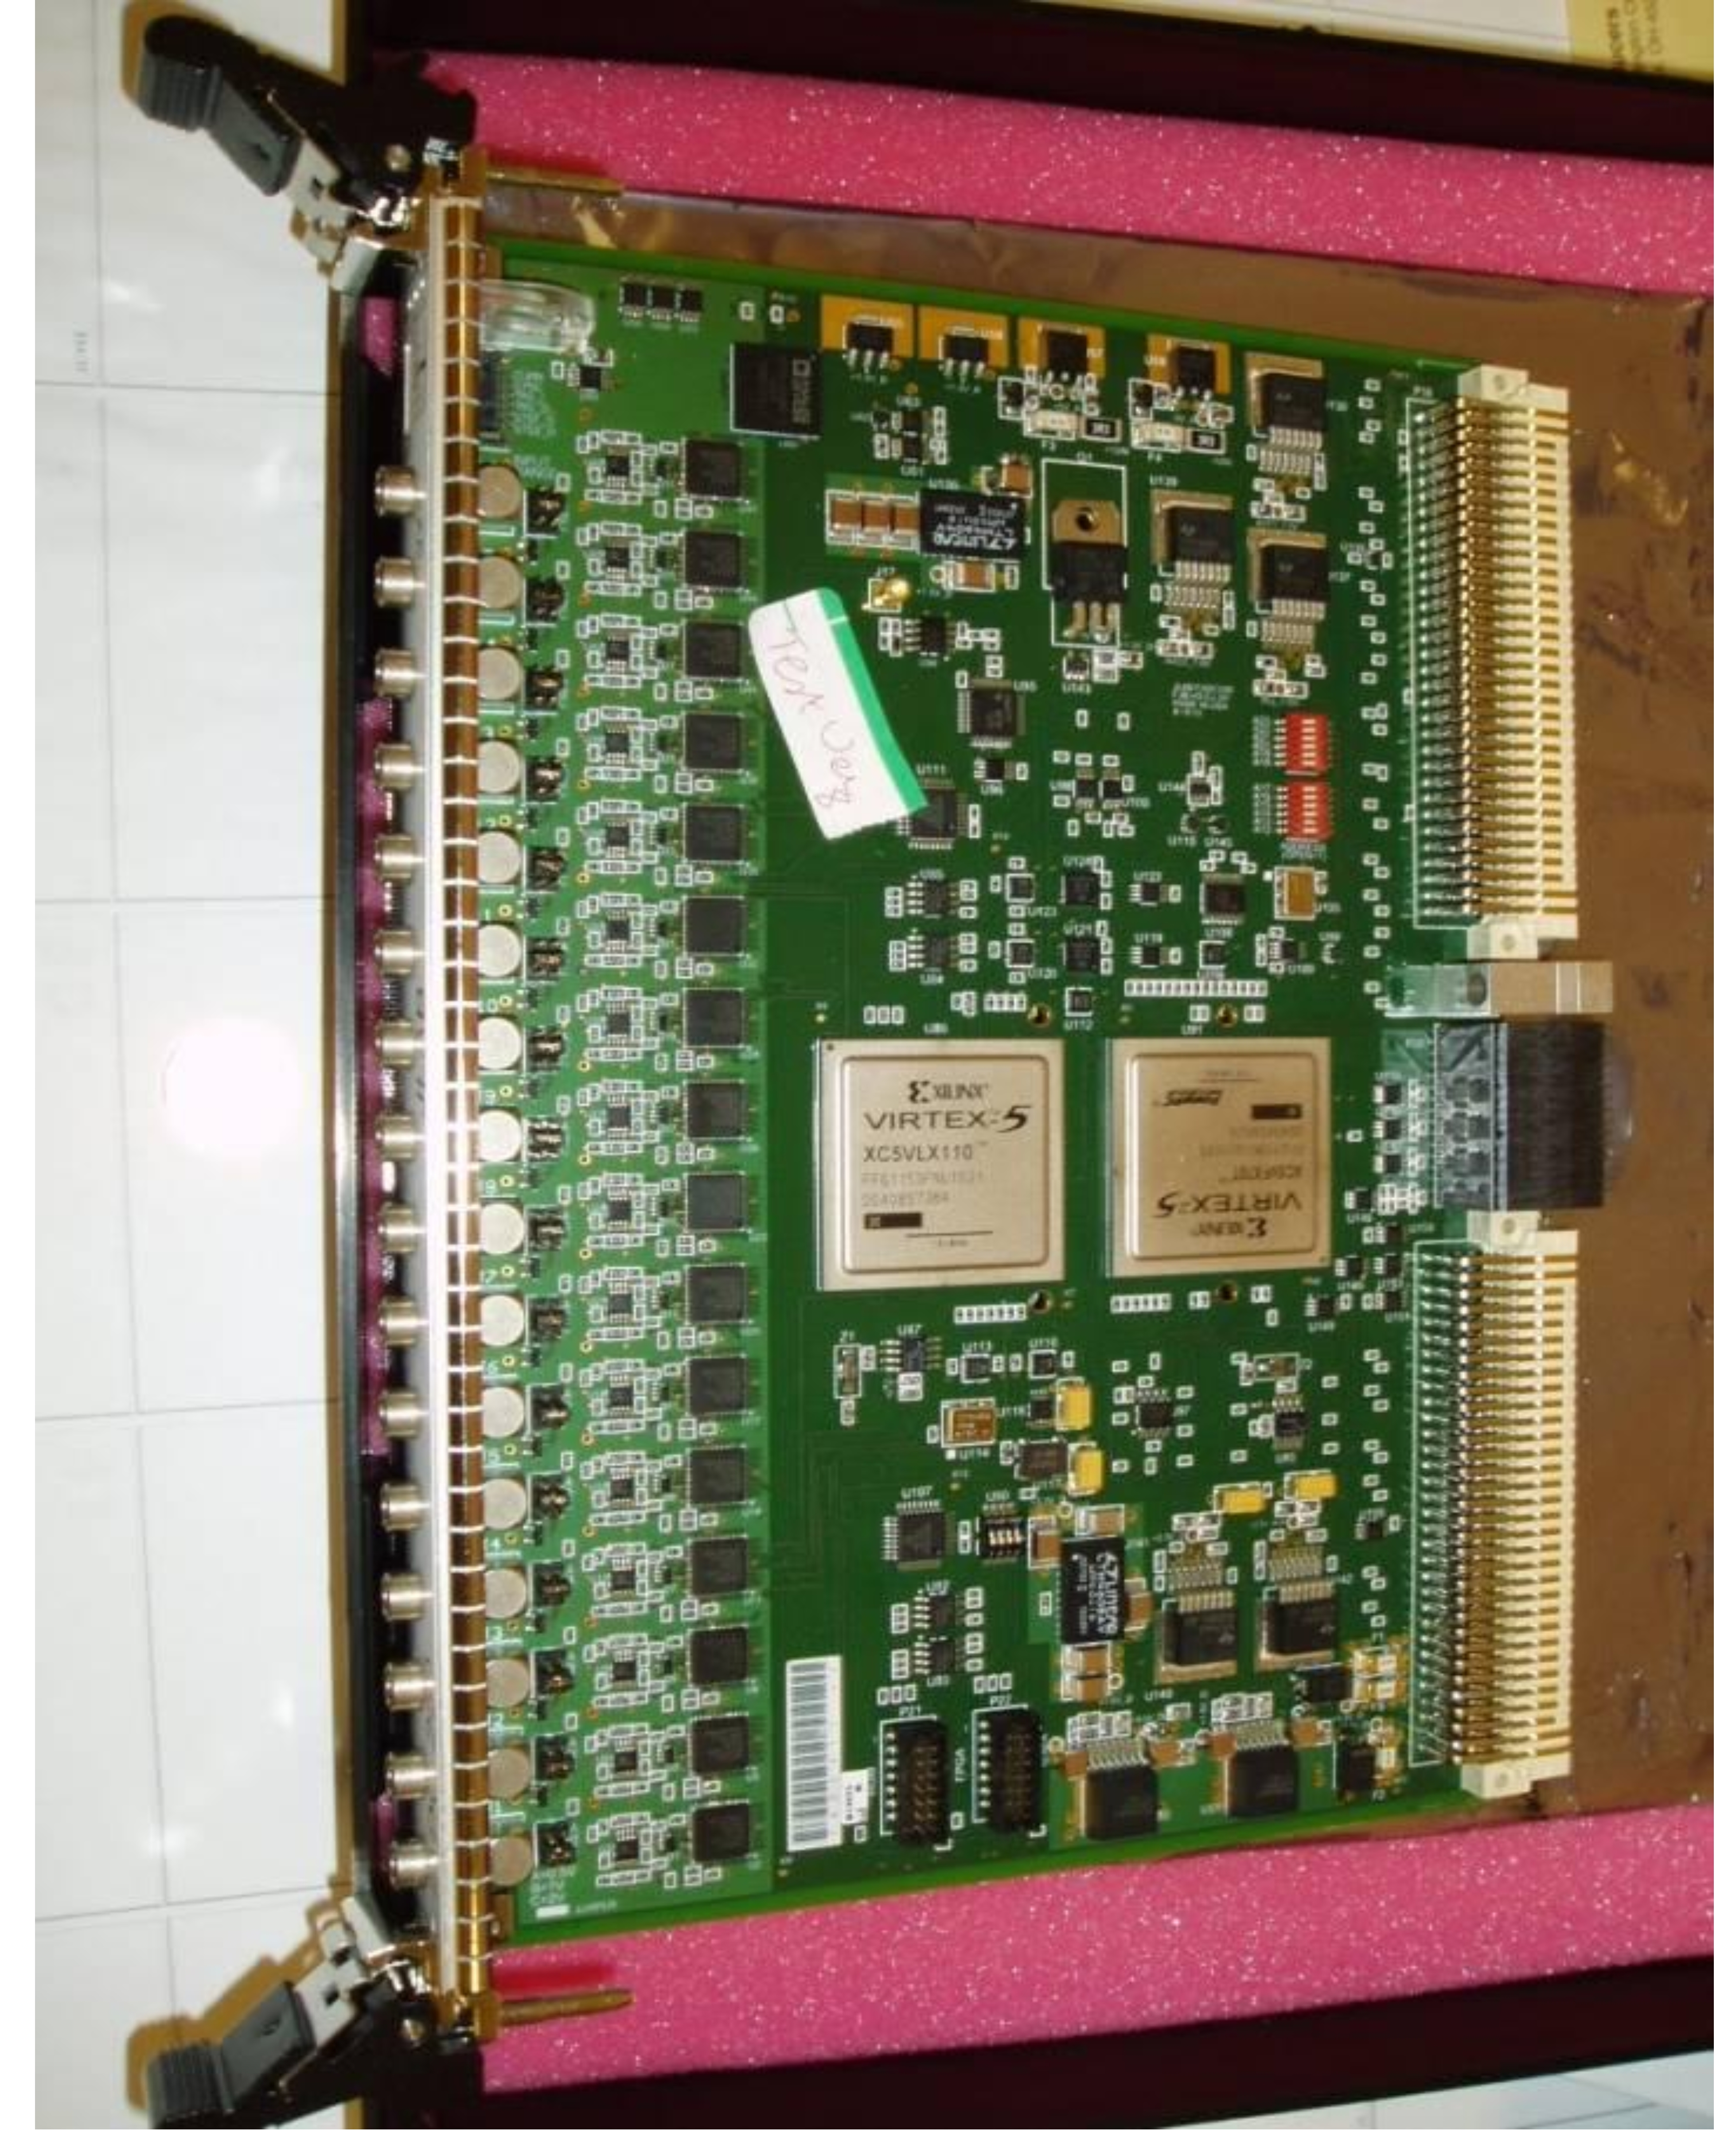
\includegraphics[width=7cm]{figures/FADC250_Photo_001.jpg}
\caption{A Jefferson Lab FADC250 VXS module.}
\label{fig:fadc}
\end{figure}
}
\end{center}
Three 20-slot VXS crates are needed to accommodate the system: one for each half of the ECal with 221 
channels and one for the Muon System with a total of 232 channels. 

The FADCs store 12-bit digitized samples at 250~MHz in 8~$\mu$s deep pipelines. 
When a trigger is received, the appropriate part of the pipeline is accessed. If a FADC   
signal exceeds a predefined threshold within that time window, the integrated amplitude of a pre-defined 
number of samples before (NSB) and after (NSA) the signal passed threshold, in addition to the time, are 
recorded. 
%as explained in Fig.~\ref{fig:hps_trigger_data}. 
This scheme significantly compresses the data input 
to the FADC. During data analysis, a pedestal value is subtracted to obtain the actual summed energy.
The main characteristics of the FADC are:
\begin{itemize}
\item 12-bit digitizer with sampling rate of 250~Msps, 
\item 50$\Omega$ termination input, 
\item front-end input range:  -0.5V, -1V or -2V (sufficient to avoid signal clipping for large pulse heights),
\item nominal charge resolution between 10-39~fC per ADC (see Tab.~\ref{tab:charge_resolution}).
\end{itemize}
\begin{center}
{\small
\begin{table}[h]
\centering
\begin{tabular}{|c|c|}
\hline
Input range & Nominal charge resolution\\
(V) & (fC per ADC count)\\\hline
-0.5 & 9.76  \\\hline
-1.0 & 19.53  \\\hline
-2.0 & 39.06 \\\hline
\end{tabular}
\caption{Nominal FADC charge resolution for different front-end input ranges.}
\label{tab:charge_resolution}
\end{table}
}
\end{center}
As shown in Fig.~\ref{fig:hps_trigger_data}, the FADC has two parallel data paths: the readout and trigger paths. The trigger path runs continuously to report hits to the trigger system. The readout path only reports hits to the DAQ when the FADC receives a trigger.

For the readout path, every FADC has the following parameters:
 \begin{itemize}
 \item the number of samples integrated before the signal crossed threshold ($NSB$), 
 \item the number of samples integrated after the signal crossed threshold ($NSA$),
 \item the readout threshold, measured in ADC counts.
 \end{itemize}
The number of samples for a given channel integration is the sum of $NSB+NSA$ samples. It is a fixed gate width pulse integration with no pedestal subtraction where the sum is stored in a 17-bit register for readout (pedestal subtraction happens offline). 
\begin{center}
{\small
\begin{figure}[]
\includegraphics[width=7cm]{figures/hps_trigger_data}
\caption{\small{FADC data paths}}
\label{fig:hps_trigger_data}
\end{figure}
}
\end{center}
For the trigger path, every channel has, in addition to $NSB$ and $NSA$: 
\begin{itemize}
% \item number of samples integrated before the threshold crossing (NSB),
 %\item number of samples integrated after the  threshold crossing (NSA),
 \item trigger threshold, measured in ADC counts, 
 \item a pedestal, 
 \item a conversion factor (gain) that converts the ADC counts to energy in MeV (with 13 bits:  from 0 to 8191~MeV), 
 \item an energy discriminator threshold (minimum energy cutoff).
 \end{itemize}
Note that the threshold for the trigger path can be set independently from the readout threshold.
The pedestal value is subtracted from the integrated sum over $NSB+NSA$ samples and 
converted to MeV units using a supplied gain conversion factor. The energy discriminator can be used to cut 
off low energy pulses before reporting to the Crate Trigger Processor. 
The values reported to the Crate Trigger Processor are the 13-bit pulse energy and the time at which the 
pulse crossed the threshold. Data for every channel is sent every 32~ns (if there is no hit a 0 energy pulse is 
sent) which sets a worst case double pulse resolution of 32~ns for individual channels, but less if pulses 
occur in adjacent 32~ns windows.

\subsubsection{Trigger Boards}
Describe CTP and SSP?


\subsection{Trigger}
\label{sec:trigger}
The trigger system is designed to efficiently select \ee{} events by 
using information from the ECal . The trigger looks for time coincidences of clusters in the top and bottom half 
of the ECal.  The trigger system can be broken down into three sections (see Fig.~\ref{fig:hps_trigger_cal}):
 \begin{itemize}
 \item FADC (pulse finding): samples and digitizes the signal pulses from each detector channel. Sends the measured pulse energy and arrival time to the CTP.
\item CTP (cluster finding): groups FADC pulses from each half of the ECal into clusters. The cluster energy, arrival time, and hit pattern are sent to the SSP.
 \item SSP (cluster pair finding): searches for time coincidence of pairs of clusters from the top and bottom half of the ECal and applies topological selections.
 \end{itemize}
\begin{center}
{\small
 \begin{figure}[t]
 \includegraphics[width=7cm]{figures/hps_trigger_cal}
\caption{Block diagram of the ECAL trigger system consisting of the FADC that samples and digitizes the detector channel signals and sends them for cluster finding in the CTP. The CTP clusters are sent to the SSP where the final trigger decision is taken based on pairs of clusters in both halves of the ECal. The decision is sent to the Trigger Supervisor (TS) that generates the necessary signals to readout the sub-detectors.}
 \label{fig:hps_trigger_cal}
 \end{figure}
}
\end{center}
The time coincidence window of pairs of clusters in the top and bottom half of the ECal are programmable 
with 4~ns resolution. 



As described above in Sec.~\ref{sec:fadc}, the first stage of the trigger logic is incorporated into the 
FPGA's on the FADC boards which sends crystal energy and time information to the CTP. With the available 
3-bit time information, the CTP looks for time coincidence of crystal signals with 8~ns resolution (limit is 4~ns).
The cluster finding algorithm is very fast and makes use of the parallel processing nature of FPGA's by 
simultaneously searching for 125 clusters, up to 3x3 in size, across the calorimeter crystal array and performs 
the following tasks:
\begin{itemize}
\item Adds energy from hits together for every 3x3 square of channels in ECal.
\item Hits are added together if they occur (leading edge) within a programmable number of 4~ns clock cycles of each other (HPS will use 8~ns time coincidence time interval).
\item If the 3x3 energy sum is larger than the programmable cluster energy threshold and the sum is greater than any neighboring 3x3 windows, the CTP reports the cluster parameters to the SSP. 
\end{itemize}
The CTP evaluates all hits in its half of the calorimeter every 4~ns. A programmable time window is used to 
allow hits that are out of time with each other to be considered as part of a cluster sum. This is done by 
reporting hits when they occur and then reporting them again for the next $N$ number of 4~ns clock cycles, 
where $N \in [0,7]$. This is useful to deal with skew and jitter that develop from the detector, cabling, and 
electronics. As described above, the CTP only selects the 3x3 window with the highest energy sum of its 
neighbors. This filtering is applied to deal with overlapping clusters and cases where the cluster is larger than 
a 3x3 window.

 The final trigger decision is made in the CTP and Sub-System Processor (SSP). The Trigger Supervisor generates all necessary signals and controls the entire DAQ 
system readout through the Trigger Interface (TI) units. The TI units are installed in every crate that participate 
in the readout process. 

The trigger system is free-running and driven by the 250~MHz global clock and has essentially zero dead 
time at occupancies expected by HPS. The Trigger Supervisor can apply dead time if necessary, for example 
on a `busy' or `full' condition from front-end electronics. The system is designed to handle trigger rates above 
50~kHz and a latency set to $\approx 3~\mu$s to match that required by the SVT APV25 chip. 




\subsubsection{Performance}
As discussed above, the trigger and DAQ integrate pulses differently to measure hit energy. The trigger 
integrates using a time-over-threshold window, and the DAQ readout integrates using a constant window 
(5 samples before and 30 samples after a threshold crossing). For every event, the trigger reports the 
trigger decision as a bit mask (top trigger, bottom trigger, or both) and the time the trigger fires.

We study trigger performance by simulating the trigger for each event and comparing to how events were 
actually triggered.
First, we simulate the FADC readout board to convert from readout hits (constant integration window) to 
trigger hits (time-over-threshold integration). We then simulate the CTP clustering algorithm and the trigger 
decision before we compare the trigger decision and trigger time reported by the simulation to what was 
reported by the real trigger.

To eliminate trigger bias in checking the trigger decision, we use a tag and probe method. To check trigger 
performance in one half of the ECal, we tag events where there was a trigger in the other half, and exactly one 
probe cluster in the ECal half under test. 
We then measure trigger efficiency (proportion of tagged events where there was a trigger) as a function of 
ADC counts and energy of the probe cluster.
These turn-on curves are shown for the top half of the ECal in Fig.~\ref{fig:turnon}. 
\begin{center}
{\small
\begin{figure}[ht]
	\includegraphics[width=7cm]{figures/top_turnon_adc}
	\includegraphics[width=7cm]{figures/top_turnon_e}
	\caption{Trigger turn-on as a function of probe cluster ADC counts (top) and probe cluster energy in MeV 
	(bottom). Both plots are for the top half of the ECal; bottom is similar. Energy is not corrected for sampling 
	fraction.}
\label{fig:turnon}
\end{figure}
}
\end{center}
The trigger threshold is seen to be 1280 ADC counts as expected. The threshold is not perfectly sharp in this 
analysis because of uncertainties in the conversion from readout to trigger hits but based on comparisons 
with Monte Carlo simulation we believe the trigger worked exactly as specified. 
The trigger threshold in terms of cluster energy is very uneven for two reasons; gain variations between 
different ECal crystals lead to threshold variations and the nonlinearity of the time-over-threshold integral 
means that the effective threshold is higher for clusters that span multiple crystals.
Overall the trigger appears to have functioned exactly as intended. Changes planned for the next run 
(constant integration window and per-crystal gain calibration constants for the trigger) will solve both of the 
issues that led to threshold variations in the test run.


\subsection{Data Acquisition and Online Computing}
For the ECal, every VXS crate contains a Readout Controller (ROC)
that collects digitized information, processes it, and sends it on to the Event Builder (EB). The ROC is a single 
blade Intel-based CPU module running DAQ software under CentOS Linux OS. For the SVT ATCA system, 
the ROC application runs on an embedded processor situated on the ATCA main board. The EB assembles 
information from the SVT, ECal and Muon System ROCs into a single event which is passed to the Event 
Recorder (ER) that writes it to a RAID5-based data storage system capable of handling up to 100 MB/s. The 
EB and other critical components run on multicore Intel-based multi-CPU servers. The DAQ network system is 
a Foundry router providing high-speed connections between the DAQ components and to the JLab 
computing facility. The SVT ROC, which must handle large data volumes, has a 10 Gbit/s link to the Foundry 
router, while a 1 Gbit/s link is adequate for the ECal and Muon System. A 10 Gbit/s uplink to the JLab 
computing facility is used for long-term storage.

The SVT DAQ is described in more details in Sec.~\ref{sec:svt_daq}.



%%%%%%%%%%%%%%%%%%%%%%%%%%%%%%%%%%%%%%%%%%%%%%%%%%


\section{Multiple Coulomb Scattering Distributions}

Occupancies close to the beam create many of the key challenges in the HPS experiment
and determine the limits of sensitivity to low \Aprime{} masses.
These occupancies are dominated by electrons which have multiple Coulomb scattered (MCS) 
to relatively large angles in the target. Because HPS is sensitive to scattering angles far out on the tail of the 
MCS distribution, well beyond the angles important in other experiments, care must be taken
to ensure our simulations are correct in this regime.  

\subsection{Multiple Coulomb Scattering Models}

One of the main goals of the HPS Test was to evaluate the description of the tails of the MCS
to gain further confidence in the expected detector occupancy in the full HPS experiment. 
Previous studies of multiple scattering angles show good agreement with the \moliere{} 
theory~\cite{Moliere:1948zz} for a wide range 
of materials and projectiles~\cite{Attwood:2005zz,Shen:1978ha,Gottschalk1993467}. We have verified that 
the angular distribution $F(\theta)$ in the differential cross section $d\sigma = F( \theta) d(\cos\theta) d\phi$ 
for the \egs{}~\cite{egs5} simulation program show good agreement with \moliere{}'s analytical formula as 
formulated by Bethe~\cite{Bethe:1953va}. 
The small angle approximation was also shown to be in agreement with the theory formulated by Gaudsmit and 
Saunderson~\cite{Goudsmit:1940zza,Goudsmit:1940zz} that is valid for any angle. 
While \egs{} uses the more complex and time consuming \moliere{} 
formula, \geant{} uses an approximation with two, continuously joined, functions to take into account 
small and large angle scattering. Due to the explicit function in large angle approximation used by \geant{} 
we expect that \geant{} will overestimate the angular distribution at angles larger than a few mrad.


Figure~\ref{fig:schematic_testrun_vs_erun} gives a schematic view of the main differences 
between the photon and electron beam setup. 
\begin{figure}[ht]
\includegraphics[ width=7cm]{figures/photon_vs_electron_beam_schematic.png}
\caption{\small{Schematic comparison of HPS Test run photon beam compared to the HPS electron beam.}}\label{fig:schematic_testrun_vs_erun}
\end{figure}
The angular distribution of the pair produced electron and positron emerging 
from the converter in the test run has comparable contributions from {\it i)} the pair production angle
and {\it ii)} the MCS of the electron and positron in the converter after production. By measuring the 
scattering rate at several different converter thicknesses we can vary the contribution from MCS 
while the contribution from the pair production angle is constant. This allows us to confirm our model of MCS 
despite the fact that all data was taken with a photon beam.


\subsection{Running Conditions}

Data was taken at three different converter thicknesses with a beam current varying between 
$30-70$~nA, see~Tab.~\ref{tab:currents}.  The photon beam line during the test run produced a relatively 
large fraction of pairs 
originating upstream of the converter. This contribution was measured during data taking 
with ``empty'' converter runs i.e. removing the converter but with all other conditions 
the same. 
The upstream background measured in the ``empty'' converter runs was subtracted 
from the other runs, properly normalized using the measured integrated currents.
\begin{table}
\begin{center}
{\small
\begin{tabular}{|c|c|c|}
\hline
Converter thickness & Duration &  $e^-$ on converter \\
 (\%$X_0$) & (s) & (nC)    \\   
\hline
%\hline
1.6   & 911 &     24385.9     \\ %27 nA
%\hline
0.18   & 2640 &    193508.9  \\  %73 nA
%\hline
0.45  & 2149 &       140709.9  \\ %65.5 nA
%\hline
0    & 1279  &   88079.6  \\
\hline
\end{tabular}
\caption{Measured integrated currents for the dedicated photon runs.}
\label{tab:currents}
}
\end{center}
\end{table}


\subsection{Measured Angular Distributions}


We measure the vertical angular distributions of electrons and positrons using the ECal. 
Cluster reconstruction and calibration was performed as described in Sec.~\ref{sec:ecal}. The measured 
angular distribution in the ECal for the three converter thicknesses are shown in 
Fig.~\ref{fig:ang_distr_data} (left).  
\begin{center}
{\small
	\begin{figure}[]
	\includegraphics[ width=7cm]{figures/rate_ecalrow_raw.png}
	\includegraphics[ width=7cm]{figures/rate_ecalrow_norm_subtr.png}
	\caption{Measured raw vertical angular distributions before (top) and after (bottom) 
	normalization and background subtraction.}
	\label{fig:ang_distr_data}
	\end{figure}
}
\end{center}
The background fraction for the three converter thicknesses was 16\%, 52\% and 71\% 
for converter thicknesses of 1.6\%, 0.45\% and 0.18\%, respectively. The background fraction was also 
cross-checked by pointing back tracks reconstructed in the SVT to identify the fraction of tracks not originating 
from the converter. We also checked that the contribution from photons to our triggered 
sample was much less than 2\%. These measured angular distributions are compared to simulation to validate 
the modeling of the MCS. \egs{}~\cite{egs5} is used to generate 
the electromagnetic interactions in the converter while \geant{} is used to simulate the particles after the 
converter.  Figure~\ref{fig:ang_distr_dataMC} shows the angular distribution comparing data and 
\egs{} normalized to 1~s of beam at 90~nA beam current. Taking into account systematics uncertainties 
described below reasonable agreement is obtained;   total rates for each converter thickness is shown in 
Fig.~\ref{fig:rate_vs_thickness} and summarized in Tab.~\ref{tab:ang_distr_dataMC}.
\begin{center}
{\small
	\begin{figure*}[t]
	\includegraphics[ scale=0.25]{figures/dataMC_1351_Hit_Y_top_norm_bkgsub.png}
	\includegraphics[ scale=0.25]{figures/dataMC_1354_Hit_Y_top_norm_bkgsub.png}
	\includegraphics[ scale=0.25]{figures/dataMC_1353_Hit_Y_top_norm_bkgsub.png}
	\caption{Comparison between the observed and predicted angular 
distribution using \egs{} for a converter thickness of 1.6\% (left), 0.45\% (middle) and 0.18\% 
(right).  Only statistical uncertainties are shown. }
	\label{fig:ang_distr_dataMC}
	\end{figure*}
}
\end{center}
\begin{center}
{\small
	\begin{figure*}[t]
	\includegraphics[ scale=0.3]{figures/dataMC_geant4.png}
	\includegraphics[ scale=0.3]{figures/dataMC_egs.png}
	\caption{\small{The measured rate as a function of converter thickness comparing \geant{} (left) 
	and \egs{} (right)}.} 
	\label{fig:rate_vs_thickness}
	\end{figure*}
}
\end{center}
The total systematic uncertainty was estimated to be between 10-18\% depending on the run, they include:  
uncertainty on the integrated current normalization (5\%), alignment of the ECal, uncertainty from the 
background normalization and limited Monte Carlo statistics.  
\begin{table}
\begin{center}
{\small
\begin{tabular}{|l|c|c|c|}
\hline
Converter (\% $X_0$) & 1.60 & 0.45 &	0.18 \\
\hline
\egs{} &	1162 $\pm$ 112 &	255 $\pm$ 28 &	94 $\pm$ 17	\\
\hline
\geant{} & 2633 $\pm$ 250 & 	371 $\pm$ 38 &	114 $\pm$ 18 \\
\hline
Observed 	& 1064 $\pm$ 2 & 196 $\pm$ 1 &	92 $\pm$ 1 \\						
\hline
\end{tabular}
\caption{ Observed and predicted number of events for 1~s of beam at 90~nA for three different converter 
thicknesses. The uncertainty on the prediction includes systematic uncertainties. }
\label{tab:ang_distr_dataMC}
}
\end{center}
\end{table}

\subsection{Conclusion}
In summary, the accurate modeling of the MCS is fundamental to estimate occupancies and trigger rates 
for HPS. \egs{} predicts the correct angular distribution across all converter thicknesses while 
\geant{} overestimates the rates; with the disagreement increasing  with larger converter thickness. 
This preliminary result verifies similar studies [] and gives confidence in our modeling of the MCS 
using \egs{} for evaluating the physics reach of HPS.




%%%%%%%%%%%%%%%%%%%%%%%%%%%%%%%%%%%%%%%%%%%%%%%%%%


\section{Summary}

This paper reviewed the HPS Test run apparatus, a simplified version of that 
planned for the full HPS experiment, and demonstrates the feasibility of the detector
technologies proposed for the silicon vertex tracker, the electromagnetic calorimeter, data acquisition and 
trigger systems and their performance. Of particular importance, data from dedicated photon beam running has 
been used to compare
the observed trigger rates with that expected in simulation. The trigger rate is almost entirely due to
photons which have converted to \ee{} upstream of the HPS Test setup and is sensitive to the multiple
Coulomb scattering of electrons and positrons in the conversion target.  Since scattered primary beam is 
the dominant source of occupancy in running HPS in an electron beam, good agreement between data and 
simulation confirm the background simulation used to benchmark the physics reach of the HPS experiment. 

In addition to this important test of our background simulation, the HPS Test run accomplished the following 
goals:
\begin{itemize}
	\item More than 97\% of the SVT channels functioned properly
	\item SVT readout signal to noise of XXXX, required to achieve the expected spatial and temporal resolutions
	\item SVT hit time resolution of 2.6~ns, proving hit time reconstruction will work for HPS
	\item SVT hit efficiency greater than 98\%
	%\item SVT track reconstruction efficiency greater than 98\%
	\item Survey-based SVT alignment performed as expected and will allow track-based alignment
	\item 87\% of ECal crystals functioned properly, with defects to be corrected by planned ECal upgrades
	\item The ECal has been calibrated using SVT tracks
	\item The SVT and JLab data acquisition systems were successfully integrated
	\item The trigger functioned as designed; rates greater than 100~kHz was tested in special runs
	% deficiencies found in test run trigger performance are addressed for the 2014-2015 run
\end{itemize}

While the HPS Test run successfully allowed us to test many aspects of the HPS experiment, there were 
limitations to what could be achieved in some key areas such as mass resolution and vertexing 
performance. In particular, the low statistics and lack of resonances or scattered beam electrons prohibits a 
direct analysis of the momentum resolution 
and tails of the vertex distribution. However, for both of these performance parameters, the observed 
agreement between data and simulation in key distributions supports the performance expected for the 
proposed experiment. 



%%%%%%%%%%%%%%%%%%%%%%%%%%%%%%%%%%%%%%%%%%%%%%%%%%

\section{Lessons Learned and Outlook}

In the process of developing the HPS Test design, it was found that this simple system was capable of 
delivering a surprising fraction of the physics potential anticipated for the full experiment.  With this in mind, 
we have proposed a new design for the HPS detector that builds upon the HPS Test , principally 
by addressing the compromises made for HPS Test to ensure the best possible performance for \Aprime{} 
physics within the envelope of the existing beam line layout and analyzing magnet. For the SVT, 
this design uses the same sensors, readout chips, and module concept and for the ECal the crystal and 
detector layout will be identical, retaining the most successful 
elements of the test run apparatus and addressing the weaknesses identified during assembly and 
operation. The new SVT layout adds a sixth layer for more robust tracking, adds acceptance in the 
three deeper layers to increase physics sensitivity and provides better silicon cooling to improve longevity. 
Other major updates needed for the full experiment are updates to the SVT electronics and 
DAQ; improving connectivity and cabling, moving digitization closer to the front-end electronics and 
updating the data reduction, event handling and trigger synchronization to reach 50~kHz trigger rates. 
This first generation of the full experiment will be ready to take physics data when CEBAF begins operation 
again in end of 2014.




%% The Appendices part is started with the command \appendix;
%% appendix sections are then done as normal sections
%% \appendix

%% \section{}
%% \label{}

%% References
%%
%% Following citation commands can be used in the body text:
%% Usage of \cite is as follows:
%%   \cite{key}          ==>>  [#]
%%   \cite[chap. 2]{key} ==>>  [#, chap. 2]
%%   \citet{key}         ==>>  Author [#]

%% References with bibTeX database:

\bibliographystyle{model1-num-names}
%\bibliography{<your-bib-database>}
\bibliography{hps-testrun-nim}

%% Authors are advised to submit their bibtex database files. They are
%% requested to list a bibtex style file in the manuscript if they do
%% not want to use model1-num-names.bst.

%% References without bibTeX database:

% \begin{thebibliography}{00}

%% \bibitem must have the following form:
%%   \bibitem{key}...
%%

% \bibitem{}

% \end{thebibliography}


\end{document}

%%
%% End of file `elsarticle-template-1-num.tex'.
